
\section{Implementation Issues}
\label{sec:implementation}
Although a completed and detailed floorplan of the node is not the
focus of this work, in this section we want to give a basic idea of
which are the main elements required to support this kind of
architecture and the DiSR approach. There are three main classes of
node elements:
\begin{itemize}
\item Node-specific: components (such ALUs, memories) that are
strictly related to the node functionality and role inside a given
networks: e.g. is that a computation or storage node.
\item Node communication:  these are elements (such as transceivers,
buffers) required to the node to communicate with its neighbours,
independently from node functionality and DiSR implementation
\item DiSR-specific: all the hardware, such as control logic and
configuration, required to implement the proposed DiSR approach.
\end{itemize}


Let us now look inside the \emph{DiSR} block which implements the DiSR-specific
operation. In Fig.~\ref{fig:implementation} we shown a possible sketch of this 
last one, which mainly consist in the following building blocks:

\begin{itemize}
\item \emph{DBS block}: This block take trace of the dynamic behaviour status (DBS). 
      How discussed in the Sec.~\ref{ssec:disr_dstruct}, there are six possible status. 
      These status can be codified using only 3 bit implemented with a 3-bit register 
      and the required combinatory logic. This block is essentially designed as a state machine.
\item \emph{LED register}: Is a set of register useful as storage for local environment data (LED)
      described in Sec.~\ref{ssec:disr_dstruct}. In Fig.~\ref{fig:implementation} in their 
      respective block, are highlighted two table that represents the link\_visited 
      and link\_tvisited array. The implementation of this block is an array of register 
      (one for each direction) that can be implemented with an SRAM, in which are presents two 
      specific fields  for representing the segID (nodeID+linkID). 
\item \emph{Control circuitry}: This circuitry read the information from the incoming packet, 
      LED registers and the dynamic behaviour status (DBS block) and is able to write The LED
      informations and change the dynamic behaviour status. The output (Ctrl out), drive 
      the others communications resources (such as node transceivers) for actuating the DiSR 
      routing operation.
\end{itemize}

One of the main design challenge typical of DNA Self-Assembled systems is due to the
reduced available resource (such as the number of CNFET per node) for implementing both 
computations and routing decisions for each node. Considering the budget of $10^4$ CNFET 
for each network's node\cite{liu_jetcs} we must estimate the required resource useful 
for implementing the entire DiSR block (Fig.~\ref{fig:implementation}). For this purpose, 
after a description of the DiSR circuitry with an hardware description language (VHDL) 
we have synthesized at gate-level the required hardware. Furthermore, considering the 
specific layout of each single logic elements (such as NAND, full-adder, latch etc.), 
we are able to count the number of CNFET necessary for implementing the DiSR logic. 
With this approach we estimated 2452 CNFET for implementing that blocks which constitutes 
about the 25\% of the overall node budget. This number of resource can be certainly reducing 
applying more effort in the circuitry design of each building block exposed in this section.

\begin{figure}
  \centering
  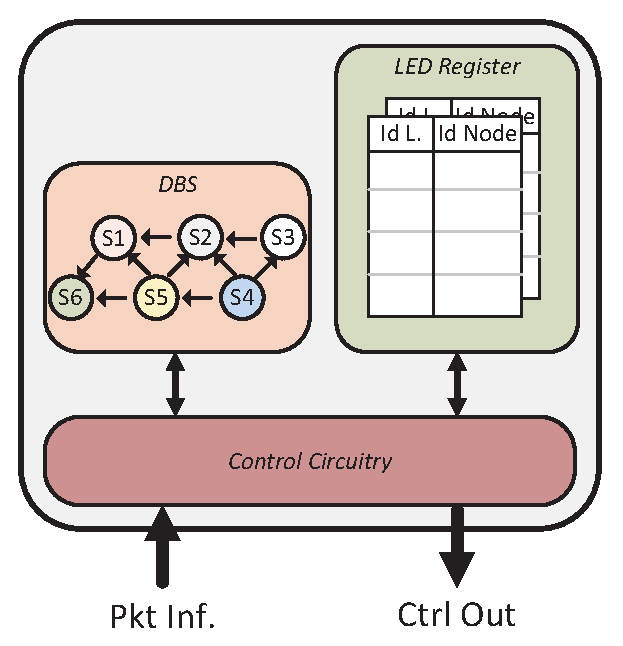
\includegraphics[width=0.40\textwidth]{pictures/disr_imp.eps}
  \caption{\emph{DiSR} block architecture.}
 \label{fig:implementation}
\end{figure}